\documentclass[11pt]{article}
\usepackage{color} %used for font color
\usepackage{amssymb} %maths
\usepackage{amsmath} %maths
\usepackage{bm}
\usepackage{epsfig}
\usepackage{soul}
\usepackage{subcaption}
\usepackage{listings}
\usepackage{authblk}
\usepackage{float}
\usepackage{graphicx}
\usepackage{multicol}
\usepackage{lipsum}
\topmargin-.5in
\textwidth6.6in
\textheight9in
\setlength{\columnsep}{0.6cm}
\oddsidemargin0in
\setlength\parindent{0pt}

%\def\fs{\scriptsize}
\usepackage{listings}
\usepackage{xcolor}

%New colors defined below
\definecolor{codegreen}{rgb}{0,0.6,0}
\definecolor{codegray}{rgb}{0.5,0.5,0.5}
\definecolor{codepurple}{rgb}{0.58,0,0.82}
\definecolor{backcolour}{rgb}{0.95,0.95,0.92}

%Code listing style named "mystyle"
\lstdefinestyle{mystyle}{
  backgroundcolor=\color{backcolour},   commentstyle=\color{codegreen},
  keywordstyle=\color{magenta},
  numberstyle=\tiny\color{codegray},
  stringstyle=\color{codepurple},
  basicstyle=\ttfamily\footnotesize,
  breakatwhitespace=false,         
  breaklines=true,                 
  captionpos=b,                    
  keepspaces=true,                 
  numbers=left,                    
  numbersep=5pt,                  
  showspaces=false,                
  showstringspaces=false,
  showtabs=false,                  
  tabsize=2
}

%"mystyle" code listing set
\lstset{style=mystyle}

\title{ \bf{Assignment II \\ MA797: Special Topics in Machine Learning}}
\author{Alp Tezbasaran$^{a}$}
\affil{\textit{$^{a}$Department of Nuclear Engineering NCSU, alptezbasaran@ncsu.edu}}
\date{October 4, 2019}
\begin{document}
\maketitle

\section{Perceptron Class}
The following introduction section describes the perceptron training code. The algorithm is implemented in Python language by using object oriented programming.\medskip

\begin{lstlisting}[language=Python, caption=Perceptron Class]
class Perceptron:

  import numpy as np

  def __init__(self, X, y, plot_data_lines = False, plot_errors = False):

    X = np.insert(X, X.shape[1], 1, axis = 1) # Insert 1s to 0th column
    self.X = X
    self.y = y.reshape(len(y),1)
    self.plot_data_lines  = plot_data_lines
    self.plot_errors = plot_errors

  def predict(self, X):
    if X.shape[1] != self.w.shape[0]: X = np.insert(X, X.shape[1], 1, axis = 1) # Insert 1s to 0th column
    predicted = np.sign(np.dot(X,self.w))
    predicted = predicted[:, np.newaxis]
    return(predicted)

  def error(self,y_pred,y_test):
    y_test= y_test.reshape(len(y_test),1)
    print(y_test.shape)
    print(y_pred.shape)
    error = float(np.count_nonzero(y_pred-y_test)) / float(len(y_test))
    accuracy = 1 - error
    return(error, accuracy)

  def train(self, w, eta = 1, epochs = 20):
    self.w = w
    if self.plot_data_lines or self.plot_errors:
      new_figure = Plotter()
      if self.plot_data_lines:
        ax = new_figure.plot_data(self.X, self.y)
        new_figure.plot_lines(0, self.X, self.y ,self.w,ax , epochs)

    accuracy = []

    for t in range(epochs):
      for i, x in enumerate(self.X):
        if (np.dot(self.X[i], self.w)*self.y[i]) <= 0:
          self.w = self.w + eta*self.X[i]*self.y[i]
      if self.plot_data_lines: new_figure.plot_lines(t+1,self.X, self.y, self.w,ax, epochs)
      y_pred = self.predict(self.X)
      accuracy.append(1-float(np.count_nonzero(y_pred-self.y)) / float(len(self.y)))
    if self.plot_errors: new_figure.plot_error(accuracy, eta)
    return(self.w)
\end{lstlisting}

The class uses 'numpy' arrays for inputs and outputs. There are 4 methods of the class defined. \medskip

$\_\_$init$\_\_$ functions is used to initialize the class where it takes arguments from the code and in this case the arguments are features $X$, labels $y$ and keyword arguments for plotting data and accuracy flags. The training data is added one column of 1s to include bias coefficients.\medskip

The next method is the predict method of the \emph{Perceptron} class which basically is the dot product (linear model) of the weights and the given data. Returns the classes. There is one column data manipulation which is used to add bias coefficients if they are not already there. During the training, the training matrix is passed to the this function. But after training is over, this method can be used to predict classes with other testing data as well. The trained weights will be stored within the object created from the class. \medskip

The method, or function \emph{error} is used to calculate accuracy and error values with given features and labels. Similar to the prediction function during training this function is used to calculate accuracy scores but also can be used individually to calculate error and accuracy using label from prediction and testing set.\medskip

Last method of the class is \emph{train} which takes positional arguments of eta (the learning rate) and number of epochs. They are positional arguments that means they have a predefined value, making it optional to pass those arguments. Initial weights, $w$, however is required. The method first initializes the weights from the given argument (initial weights), then plots the data if a graph is desired. Actual training begins with the for loop where t changes in range of epochs. The training data, $X$ is iterated througout all the observations, and weights are updated based on the \underline{gradient descent} algorithm. This is basically checking if the prediction is lower than 0 and updating the weights if the answer is yes. The rest of the function is to store scores (this case accuracy), and returning the weights that represents the best hyperplane. \medskip

The accuracy is used as the metric of success for the classifiers trained in this study which is defined as;
$$
Accuracy = \frac{lenght(y_{test} == y_{prediction})}{N_{samples}}
$$
This metric is sometimes called score (scikitlearn perceptron for example) and it is the universal measure of performance.

\section*{1) Perceptron Learning Model} 

\subsection*{a)} Plot the data points that to observe they are linearly separable. 

\begin{align*}
    &C_1 (1): \quad (0, 1.5)^T \ (1, 1)^T \ (2, 2)T \ (2, 0)^T \\
    &C_2 (-1): \quad (0, 0)^T \ (1, 0)^T \ (0, 1)^T
\end{align*}

\begin{figure}[H]
\centering
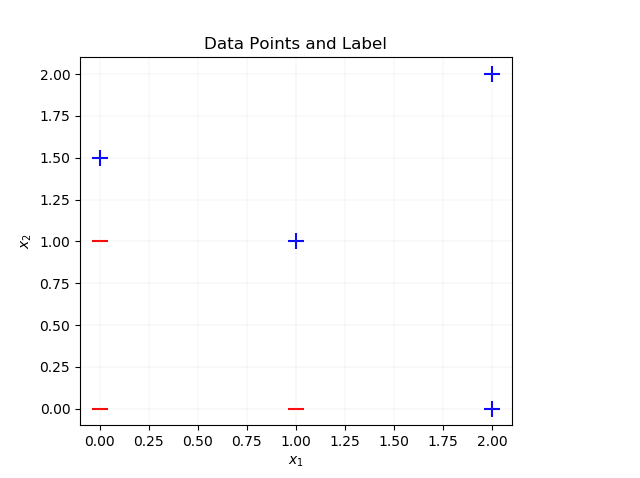
\includegraphics[width=0.75\columnwidth]{pics/a2_q1_a.png}
\captionsetup{justification=centering}
\caption{Data Points and Labels}
\label{fig:q1a}
\end{figure}

It is clear that this 2-dimensional data is linearly separable, in other words, there is a hyperplane (a line in 2-dimensional space) that can distinguish two classes.

\subsection*{b)} Plot the linear model $w^T X = 0$. The weights are;
$$
w = (-2, 4, 1)^T
$$
Here $w_0 = -2$ is the threshold with corresponding $X_0 = 1$.

\begin{figure}[H]
\centering
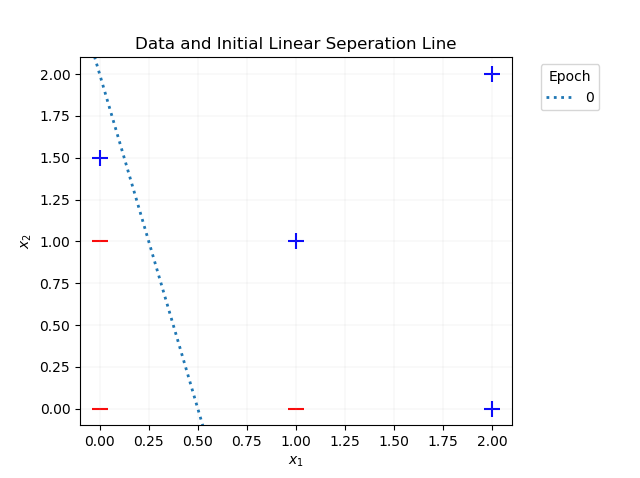
\includegraphics[width=0.75\columnwidth]{pics/a2_q1_b.png}
\captionsetup{justification=centering}
\caption{Data Points and Labels with Initial Linear Model}
\label{fig:q1b}
\end{figure}

Figure \ref{fig:q1b} clearly shows that the suggested linear model does not separate the two classes properly.

\subsection*{c)} Perceptron learning algorithm to update weights to find a linear model that can separate the given data. \medskip

The perceptron algorithm has run for 10 epochs with the leaning rate of, $\eta = 1$ and the initial weight specified in the section \textbf{b}. The linear model in each iteration (epoch) is shown below. \newpage

\begin{multicols}{2}

\begin{figure}[H]
\centering
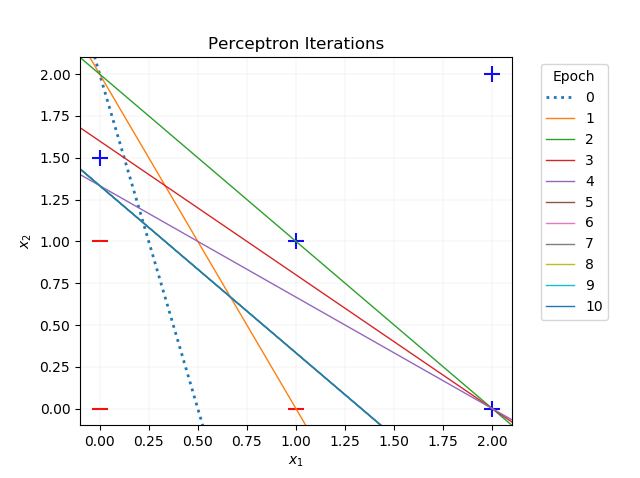
\includegraphics[width=\columnwidth]{pics/a2_q1_c.png}
\captionsetup{justification=centering}
\caption{Linear Model for each epoch}
\label{fig:q1c}
\end{figure}

\begin{figure}[H]
\centering
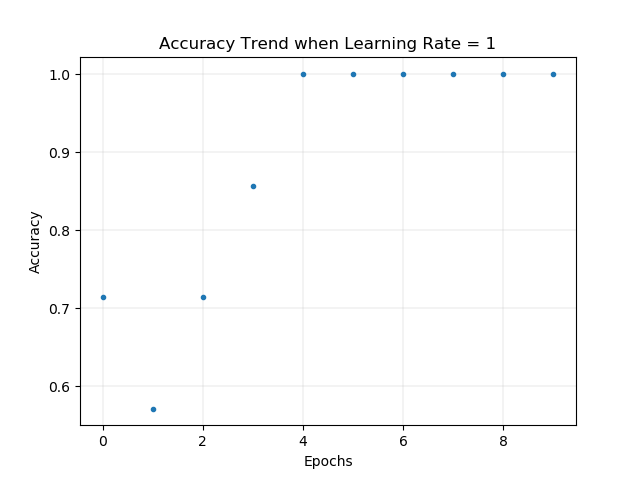
\includegraphics[width=\columnwidth]{pics/a2_q1_c2.png}
\captionsetup{justification=centering}
\caption{Training accuracy change at each epoch}
\label{fig:q1c2}
\end{figure}

\end{multicols}

And the weights calculated by the algorithm is listed in Table \ref{q1weights}. 

\bgroup
\def\arraystretch{1.5}%  1 is the default, change whatever you need
\begin{table}[H]
\centering
\caption{Weights for each epoch and accuracy estimates}
\begin{tabular}{|c|c|c|c|c|}
\hline
\textbf{Epoch}   & \ $w_0$ \  & \ $w_1$ \ & \ $w_2$ \ & \textbf{Accuracy$\%$} \\ \hline
0 &-2.0 &4.0 &1.0 & 71.43 \\ \hline
1 &-3.0 &3.0 &1.5 & 57.13 \\ \hline
2 &-4.0 &2.0 &2.0 & 71.43 \\ \hline
3 &-4.0 &2.0 &2.5 & 85.71 \\ \hline
4 &-4.0 &2.0 &3.0 & 100.0\\ \hline
5 &-4.0 &3.0 &3.0 & 100.0\\ \hline
6 &-4.0 &3.0 &3.0 & 100.0\\ \hline
7 &-4.0 &3.0 &3.0 & 100.0\\ \hline
8 &-4.0 &3.0 &3.0 & 100.0\\ \hline
9 &-4.0 &3.0 &3.0 & 100.0\\ \hline
10&-4.0 &3.0 &3.0 & 100.0\\ \hline
\end{tabular}
\label{q1weights}
\end{table}
\egroup

The table above also includes accuracy in percentage of the predicted classes of the data. In this case all the data is used to train the perceptron so in another words, the training accuracy of 100$\%$ is achieved for the given data. \medskip

Figure \ref{fig:q1c} shows the linear model of each iteration an it can be seen the lines are coinciding on top of each other starting from the 4th epoch. Figure \ref{fig:q1c2} shows the increasing accuracy for the testing data.


\subsection*{Additional examples}

Here it is further demonstrated that the perceptron learning algorithm perform properly with various examples. \bigskip

\underline{OR gate} \medskip

Traditional OR gate is a perfect example for linearly separable data. Here $x_1$ and $x_2$ are features and $y$ is their corresponding label.
\bgroup
\def\arraystretch{1.5}%  1 is the default, change whatever you need
\begin{table}[H]
\centering
\caption{OR gate data}
\begin{tabular}{|c|c|c|}
\hline
$x_1$   & \ $x_2$ \  & \ $y$  \\ \hline
1 & 1 & 1 \\ \hline
1 & 0 & 1\\ \hline
0 & 1 & 1 \\ \hline
0 & 0 & 0 \\ \hline
\end{tabular}
\label{table:or}
\end{table}
\egroup

The trained linear model by a perceptron and corresponding accuracy changes are shown below.

\begin{multicols}{2}

\begin{figure}[H]
\centering
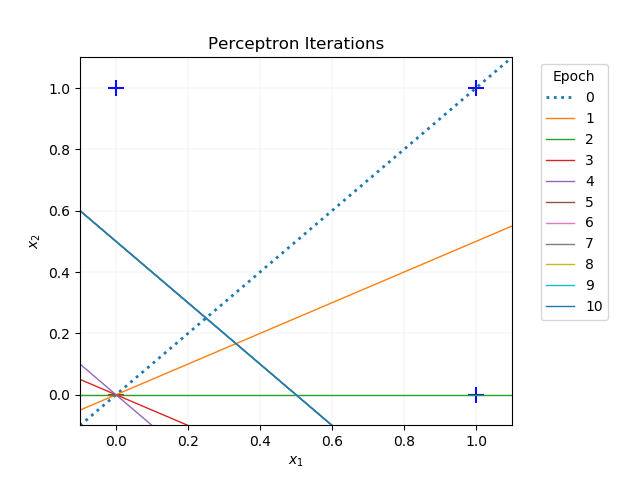
\includegraphics[width=\columnwidth]{pics/and/and.png}
\captionsetup{justification=centering}
\caption{Linear Model for each epoch}
\label{fig:or}
\end{figure}

\begin{figure}[H]
\centering
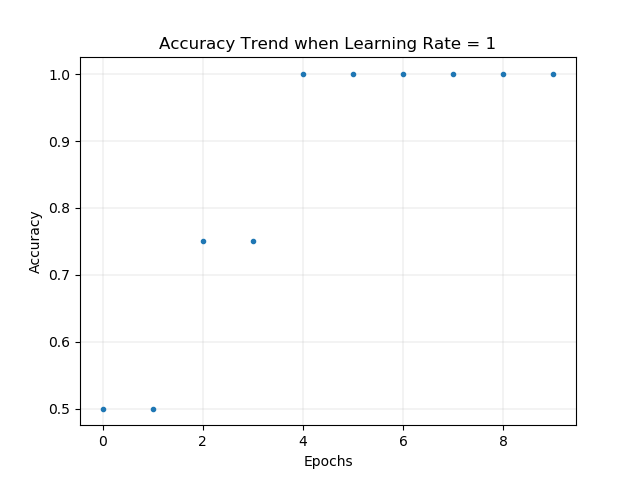
\includegraphics[width=\columnwidth]{pics/and/and_acc.png}
\captionsetup{justification=centering}
\caption{Training accuracy change at each epoch}
\label{fig:or_acc}
\end{figure}

\end{multicols}

Figures \ref{fig:or} and \ref{fig:or_acc} shows that perceptron found a separation line even when initial linear model is considerably poor. Final weights for the OR gate is $w=(-1, 2 ,2)$ \bigskip

\underline{AND gate} \medskip

Traditional AND gate is another example for linearly separable data. Here $x_1$ and $x_2$ are features and $y$ is their corresponding label same as OR gate
\bgroup
\def\arraystretch{1.5}%  1 is the default, change whatever you need
\begin{table}[H]
\centering
\caption{AND gate data}
\begin{tabular}{|c|c|c|}
\hline
$x_1$   & \ $x_2$ \  & \ $y$  \\ \hline
1 & 1 & 1 \\ \hline
1 & 0 & 0\\ \hline
0 & 1 & 0 \\ \hline
0 & 0 & 0 \\ \hline
\end{tabular}
\label{table:and}
\end{table}
\egroup

The trained linear model by a perceptron and corresponding accuracy changes are shown below.

\begin{multicols}{2}

\begin{figure}[H]
\centering
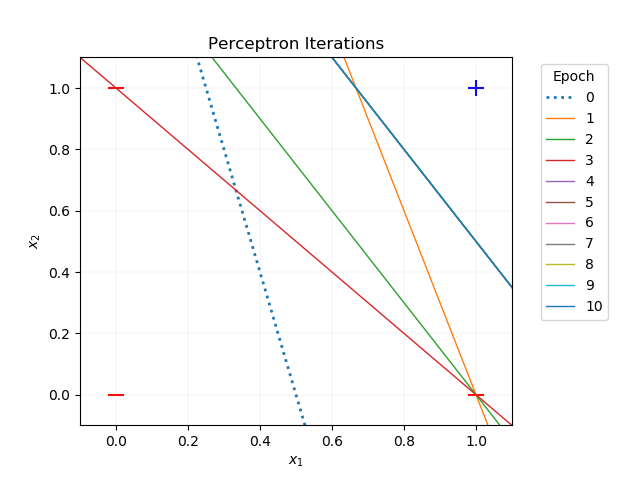
\includegraphics[width=\columnwidth]{pics/or/or.png}
\captionsetup{justification=centering}
\caption{Linear Model for each epoch}
\label{fig:and}
\end{figure}

\begin{figure}[H]
\centering
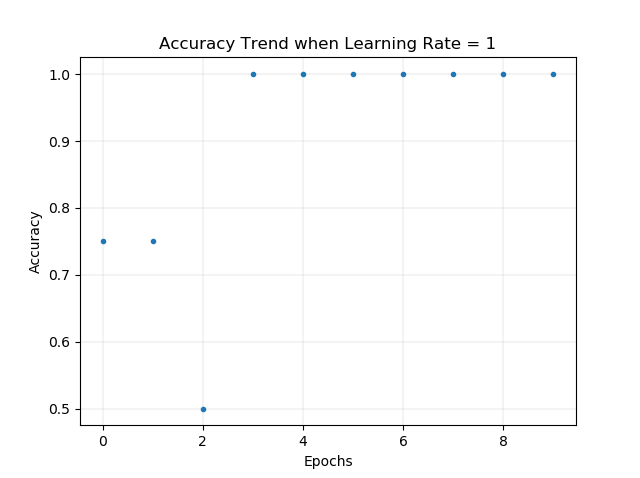
\includegraphics[width=\columnwidth]{pics/or/or_acc.png}
\captionsetup{justification=centering}
\caption{Training accuracy change at each epoch}
\label{fig:and_acc}
\end{figure}

\end{multicols}

Figures \ref{fig:and} and \ref{fig:and_acc} shows that perceptron found a separation line. The learning rate is not changed. The initial linear model was better than the OR gate so convergence required fewer epochs. Final weights for the AND gate is $w=(-4, 3 ,2)$ \medskip

Additional examples can be found with the attached code where 2-dimensional linearly separable data and labels are added. The perceptron class can be called and trained with visualization capability. The additional data can be used for further demonstration. \newpage


\section*{2) Credit application classification} 

Perceptron learning algorithm is applied to real life data which is collected from more than 600 individuals which include categorical data like gender, binary data to state if the individual is a member of the bank or not, and continuous numerical data  such as income, credit score and years of employment. The label information and data is binary and denotes if the credit application is approved or denied. Listed features are examples and there are 15 features per person and 1 label.\medskip

The goal is to train a perceptron model which will be used by the bank where when a new person applies for a credit, he or she will be classified based on the already processed applications. \medskip

The assumption for using a perceptron is that the data is linearly separable. To test this the data is divided into two sets, namely the test set and the training set. The training set is used to estimate weights, $w$, and testing data is predicted by using those weights to evaluate performance. The first 500 observations are selected as training data and the remaining is used as testing data.\medskip

To achieve the best perceptron model, two approaches are employed here. First one includes a perceptron model trained by the raw data and second one uses normalized data. The normalization is made by dividing each feature by its maximum value. Results are shown below.

\subsection*{a) Classifier trained with raw data}
The code for the perceptron is explained above. The trained model with training accuracy for each epoch is shown below. 
\begin{figure}[H]
\centering
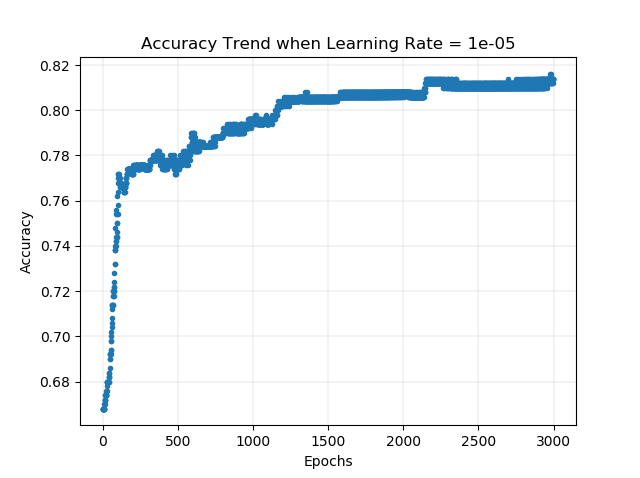
\includegraphics[width=0.75\columnwidth]{pics/q2a.png}
\captionsetup{justification=centering}
\caption{Training accuracy change at each epoch - raw data}
\label{fig:q2a_acc}
\end{figure}
One thing must be highlighted here. The original assignment states that the learning rate should be $\eta = 0.1$ and number of eopchs should be 1000. Since initial guess of the linear model is somehow important, here those values are used to estimate meta weights for the mode. Then the perceptron is trained with smaller step size (smaller learning rate) and for more epochs. Final hyperparameters are 3000 epochs and $\eta = 10^{-4}$. The scores for a perceptron with predefined values (No-tuning) are also shown. Discussions are based on the tuned model.

\bgroup
\def\arraystretch{1.5}%  1 is the default, change whatever you need
\begin{table}[H]
\centering
\caption{Accuracy of perceptron model trained with raw data}
\begin{tabular}{|c|c|c|}
\hline
Data   & \ Tuned & No-tune\\ \hline
Training & 0.830 &  0.646 \\ \hline
Testing  & 0.764 &  0.680 \\ \hline
\end{tabular}
\label{table:q2a}
\end{table}
\egroup

The trained model is used for predictions of the test set. Results are listed in Table \ref{table:q2a}, and below is sown the confusion matrix consturcted by the comparison of test set predictions to the test set labels. It is clear that initial weights has a significant effect and tuning it has its advantages. The scores improved quite substantially.

$$
cm_{test}=
 \begin{bmatrix}
 \begin{array}{rr}
86 &  13  \\
13 &  41 
\end{array}   
\end{bmatrix}
$$

Confusion matrix is basically a measure for a classifier where diagonals are correct predictions and other elements are the incorrectly predicted number of observations. As seen above there are 13 observations in the test set classified as positive o 1 that are predicted as negative or -1. Similarly there are 13 incorrect predictions of false positives. \medskip

\subsection*{b) Classifier trained with normalized data}
The following lines are used to normalize each feature with their maximum value
\begin{lstlisting}[language=Python, caption=Feature Normalizer]
 # Normalizer
  for i in range(X_train.shape[1]):
    X_train[:,i] = np.divide(X_train[:,i],max(X_train[:,i]))
\end{lstlisting}

The normalization is one the methods that are used frequently to prepare data for model construction. The idea is to make each feature more representative. Below are shown the training accuracy of the perceptron for each epoch. Here given values of $\eta = 0.1$ and 1000 epochs are used to estimate initial guess of values. Then after some tuning, final hyperparameters are selected as $\eta = 10^{-5}$ and 1000 epochs. The scores for a perceptron with predefined values (No-tuning) are also shown. Discussions are based on the tuned model.

\begin{figure}[H]
\centering
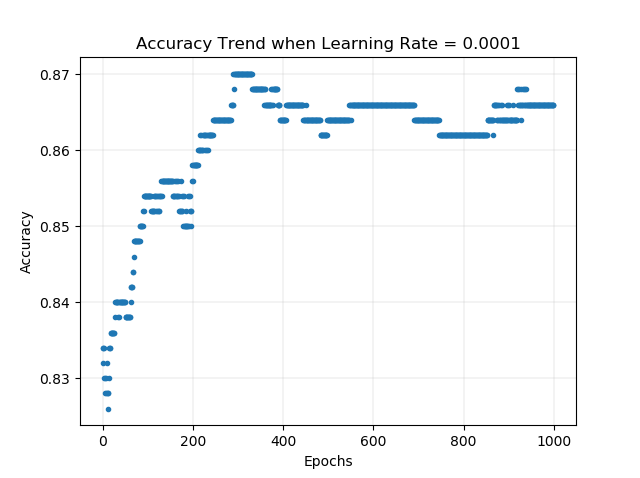
\includegraphics[width=0.75\columnwidth]{pics/q2b.png}
\captionsetup{justification=centering}
\caption{Training accuracy change at each epoch - normalized data}
\label{fig:q2_b_acc}
\end{figure}

Table \ref{table:q2b} shows the achieved accuracy levels for training and testing data.

\bgroup
\def\arraystretch{1.5}%  1 is the default, change whatever you need
\begin{table}[H]
\centering
\caption{Accuracy of perceptron model trained with raw data}
\begin{tabular}{|c|c|c|}
\hline
Data   &  Tuned & No-tune \\ \hline
Training & 0.866 & 0.849  \\ \hline
Testing  & 0.824 & 0.622  \\ \hline
\end{tabular}
\label{table:q2b}
\end{table}
\egroup

And the confusion matrix for the predictions made by the model trained with normalized data is;
$$
cm_{test}=
 \begin{bmatrix}
 \begin{array}{rr}
86 &  13  \\
14 &  40 
\end{array}   
\end{bmatrix}
$$

The discrepancy between the accuracy of training test and that of test set might be caused by the arbitrary selection of training and testing data. Selection of first 500 observations are totally random so training data might be heavily skewed on one class or might include outliers. A better approach can be a random selection from the observations, and even better approach is to conduct k-fold cross-validation where all of the observations are eventually used for test and train. \medskip

As seen there is slight improvement in the predictions but not much. These results suggest that there is further need for feature extraction or other methods for data manipulation. Additionally it is clear that this data is not linearly separable. \medskip

The referred paper in the assignment also uses linear methods to classify the highly manipulated data and their finding consists with what has been found here. Their linear classifiers (linear and quadratic discriminant analysis and no hidden layer neural network) are the worst among many. \medskip

As a final note to compare the results obtained in this study, highly verified machine learning library scikit-learn is employed. The library has a 'Perceptron' class that can be directly used. The perceptron trained with scikitlearn has a learning rate $\eta = 0.1$ and uses 1000 iterations as defined in the assignment. The training and testing scores (accuracies) are shown below.
\bgroup
\def\arraystretch{1.5}%  1 is the default, change whatever you need
\begin{table}[H]
\centering
\caption{Scikitlearn Comparison}
\begin{tabular}{|c|c|c|}
\hline
Data     & \quad  Raw   \quad & Normalized\\ \hline
Training &  60.60 & 87.80\\ \hline
Testing  &  61.44 & 86.27\\ \hline
\end{tabular}
\label{table:q2_sci}
\end{table}
\egroup

It is clear that the raw perceptron model with tuning performs significantly better than the perceptron trained with prescribed hyperparameters. On the other hand, the model constructed from normalized data has higher scores for both training and testing. This means further improvement can be made with more sophisticated tuning optimization methods.

\newpage


\underline{Note:} The full code is attached with the email where the data and plotting capabilities are included.
















\end{document}
